\documentclass[11pt,a4paper]{article}
\usepackage[margin=1in, headheight=14pt]{geometry}
\usepackage{amsfonts,amsmath,amssymb,suetterl}
\usepackage{lmodern}
\usepackage[T1]{fontenc}
\usepackage{fancyhdr}
\usepackage{float}
\usepackage[utf8]{inputenc}
\usepackage{fontawesome}
\usepackage{enumerate}
\usepackage{xcolor}
\usepackage{hyperref}
\usepackage{tikz}
\usepackage{nicefrac}
\usepackage{subcaption}

\DeclareUnicodeCharacter{2212}{-}

\usepackage{mathrsfs}
\usepackage[nodisplayskipstretch]{setspace}

\setstretch{1.5}
\renewcommand{\footrulewidth}{0pt}

\parindent 0ex
\setlength{\parskip}{1em}
\raggedbottom

\begin{document}
    %
	\begin{center}
		\vspace*{8cm}
		\Huge MA202 –Differential Equations\\
		\LARGE LECTURE 13
  \end{center}
  \newpage
  %
	\section*{Complex eigenvalues}
	\begin{itemize}
		\item We consider again a homogeneous system of n first order linear equations with constant, real coefficients,
		\begin{align*}
			x_1^\prime &= a_{11}x_1 + a_{12}x_2 + \ldots + a_{1n}x_n\\
			x_2^\prime &= a_{21}x_1 + a_{22}x_2 + \ldots + a_{2n}x_n\\
			&\quad \vdots\\
			x_n^\prime &= a_{n1}x_1 + a_{n2}x_2 + \ldots + a_{nn}x_n,
		\end{align*}
		and thus the system can be written as $x^\prime = Ax$, where
		$$
		x(t) =
		\begin{pmatrix}
			x_1(t)\\
			x_2(t)\\
			\vdots\\
			x_n(t)
		\end{pmatrix},\ A =
		\begin{pmatrix}
			a_{11} & a_{12} & \ldots & a_{1n}\\
			a_{21} & a_{22} & \ldots & a_{2n}\\
			\vdots & \vdots & \ddots & \vdots\\
			a_{n1} & a_{n2} & \ldots & a_{nn}\\
		\end{pmatrix}
		$$
	\end{itemize}
	\section*{Conjugate eigenvalues and eigenvectors}
	\begin{itemize}
		\item We know that $x = \xi e^{rt}$ is a solution of $x^\prime = Ax$, provided $r$ is an eigenvalue and $\xi$ is an eigenvector of $A$.
		\item The eigenvalues $r_1,\ \ldots,\ r_n$ are the roots of $\det(A-rI) = 0$, and the corresponding eigenvectors satisfy $(A-rI)\xi = 0$.
		\item If $A$ is real, then the coefficients in the polynomial equation $\det(A-rI) = 0$ are real, and hence any complex eigenvalues must occur in conjugate pairs. Thus, if $r_1 = \lambda + i\mu$ is an eigenvalue, then so is $r_2 = \lambda - i\mu$
		\item The corresponding eigenvectors $\xi^{(1)},\ \xi^{(2)}$ are conjugates also. To see this, recall A and I have real entries, and hence
		$$
		(A-r_1I)\xi^{(1)} = 0\ \Rightarrow\ (A-\bar{r_1}I)\bar{\xi}^{(1)} = 0\ \Rightarrow\ (A-r_2I)\xi^{(2)}=0
		$$
	\end{itemize}
	\section*{Conjugate solutions}
	\begin{itemize}
		\item It follows from the previous slide that the solutions
		$$
		x^{(1)} = \xi^{(1)}e^{r_1t},\ x^{(2)} = \xi^{(2)}e^{r_2t}
		$$
		corresponding to these eigenvalues and eigenvectors are complex conjugates as well, since
		$$
		x^{(2)} = \xi^{(2)}e^{r_2t} = \bar{\xi}^{(1)}e^{\bar{r_1}t}=\bar{x}^{(1)}
		$$
	\end{itemize}
	\section*{Real-valued solutions}
	\begin{itemize}
		\item Thus for complex conjugate eigenvalues $r_1$ and $r_2$, the corresponding solutions $x^{(1)}$ and $x^{(2)}$ are conjugates also.
		\item To obtain real-valued solutions, use real and imaginary parts of either $x^{(1)}$ or $x^{(2)}$. To see this, let $\xi^{(1)} = a+ib$. Then
		\begin{align*}
			x^{(1)} &= \xi^{(1)}e^{(\lambda + i\mu)t} = (a+ib)e^{\lambda t}(\cos \mu t + i\sin \mu t)\\
			&= e^{\lambda t}(a\cos \mu t - b\sin \mu t) + ie^{\lambda t}(a\sin \mu t + b\cos \mu t)\\
			&= u(t) + iv(t)
		\end{align*}
		where
		$$
		u(t) = e^{\lambda t}(a\cos \mu t - b\sin \mu t),\ v(t)=e^{\lambda t}(a\sin \mu t + b\cos \mu t)
		$$
		are real valued solutions of $x^\prime = Ax$, and can be shown to be linearly independent.
	\end{itemize}
	\section*{General solution}
	\begin{itemize}
		\item To summarize, suppose $r_1 = \lambda + i\mu$, $r_2 = \lambda - i\mu$, and that $r_3,\ \ldots,\ r_n$ are all real and distinct eigenvalues of $A$. Let the corresponding eigenvectors be
		$$
		\xi^{(1)} = a+ib,\ \xi^{(2)} = a-ib,\ \xi^{(3)},\ \xi^{(4)},\ \ldots,\ \xi^{(n)}
		$$
		\item Then the general solution of $x^\prime = Ax$ is 
		$$
		x = c_1u(t) + c_2v(t) + c_3\xi^{(3)}e^{r_3t} + \ldots + c_n\xi^{(n)}e^{r_nt}
		$$
		where
		$$
		u(t) = e^{\lambda t}(a\cos \mu t - b\sin \mu t),\ v(t) = e^{\lambda t}(a\sin \mu t + b \cos \mu t)
		$$
	\end{itemize}
	\section*{Example 1: Direction field (1 of 8)}
	\begin{itemize}
		\item Consider the homogeneous equation $x^\prime = Ax$ below.
		$$
		x^\prime =
		\begin{pmatrix}
			-1/2 & 1\\
			-1 & -1/2
		\end{pmatrix}x
		$$
		\item A direction field for this system is given below.
		\begin{figure}[H]
			\centering
				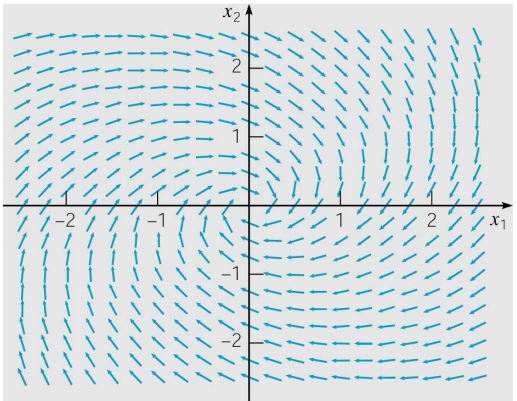
\includegraphics[width=0.45\textwidth]{figure/Lec13f1.PNG}
		\end{figure}
		\item Substituting $x = \xi e^{rt}$ in for $x$, and rewriting the system as $(A-rI)\xi=0$, we obtain
		$$
		\begin{pmatrix}
			-1/2-r & 1\\
			-1 & -1/2 - r
		\end{pmatrix}
		\begin{pmatrix}
			\xi_1\\
			\xi_2
		\end{pmatrix}=
		\begin{pmatrix}
			0\\
			0
		\end{pmatrix}
		$$
	\end{itemize}
	\section*{Example 1: Complex eigenvalues (2 of 8)}
	\begin{itemize}
		\item We determine $r$ by solving $\det(A-rI) = 0$. Now
		$$
		\begin{vmatrix}
			-1/2-r & 1\\
			-1 & -1/2-r
		\end{vmatrix}
		= (r+1/2)^2+1
		= r^2 + r + \frac{5}{4}
		$$
		\item Thus
		$$
		r = \frac{-1\pm \sqrt{1^2-4(5/4)}}{2}
		= \frac{-1\pm2i}{2} = -\frac{1}{2}\pm i
		$$
		\item Therefore the eigenvalues are $r_1 = -1/2 + i$ and $r_2 = -1/2 - i$.
	\end{itemize}
	\section*{Example 1: First eigenvector (3 of 8)}
	\begin{itemize}
		\item Eigenvector for $r_1 = -1/2 + i$: Solve\\
		$
		(A-rI)\xi = 0 \Leftrightarrow
		\begin{pmatrix}
			-1/2 - r & 1\\
			-1 & -1/2-r
		\end{pmatrix}
		\begin{pmatrix}
			\xi_1\\
			\xi_2
		\end{pmatrix} =
		\begin{pmatrix}
			0\\
			0
		\end{pmatrix}
		$\\
		$
		\Leftrightarrow
		\begin{pmatrix}
			-i & 1\\
			-1 & -i
		\end{pmatrix}
		\begin{pmatrix}
			\xi_1\\
			\xi_2
		\end{pmatrix}=
		\begin{pmatrix}
			0\\
			0
		\end{pmatrix}\Leftrightarrow
		\begin{pmatrix}
			1 & i\\
			-1 & -i
		\end{pmatrix}
		\begin{pmatrix}
			\xi_1\\
			\xi_2
		\end{pmatrix}=
		\begin{pmatrix}
			0\\
			0
		\end{pmatrix}
		$\\
		by row reducing the augmented matrix:\\
		$
		\begin{pmatrix}
			1 & i & 0\\
			-1 & -i & 0
		\end{pmatrix}\to
		\begin{pmatrix}
			1 & i & 0\\
			0 & 0 & 0
		\end{pmatrix}\to
		\xi^{(1)} = 
		\begin{pmatrix}
			-i\xi_2\\
			\xi_2
		\end{pmatrix}\to \ \text{choose}\ \xi^{(1)}=
		\begin{pmatrix}
			1\\
			i
		\end{pmatrix}
		$
		\item Thus
		$$
		\xi^{(1)} =
		\begin{pmatrix}
			1\\
			0
		\end{pmatrix} +i
		\begin{pmatrix}
			0\\
			1
		\end{pmatrix}
		$$
	\end{itemize}
	\section*{Example 1: Second eigenvector (4 of 8)}
	\begin{itemize}
		\item Eigenvector for $r_1 = -1/2 - i$: Solve\\
		$
		(A-rI)\xi = 0 \Leftrightarrow
		\begin{pmatrix}
			-1/2-r & 1\\
			-1 & -1/2-r
		\end{pmatrix}
		\begin{pmatrix}
			\xi_1\\
			\xi_2
		\end{pmatrix} = 
		\begin{pmatrix}
			0\\
			0
		\end{pmatrix}
		$\\
		$
		\Leftrightarrow
		\begin{pmatrix}
			i & 1\\
			-1 & i
		\end{pmatrix}
		\begin{pmatrix}
			\xi_1\\
			\xi_2
		\end{pmatrix}=
		\begin{pmatrix}
			0\\
			0
		\end{pmatrix}\Leftrightarrow
		\begin{pmatrix}
			1 & -i\\
			-1 & i
		\end{pmatrix}
		\begin{pmatrix}
			\xi_1\\
			\xi_2
		\end{pmatrix}=
		\begin{pmatrix}
			0\\
			0
		\end{pmatrix}
		$\\
		by row reducing the augmented matrix:\\
		$
		\begin{pmatrix}
			1 & -i & 0\\
			-1 & i & 0
		\end{pmatrix}\to
		\begin{pmatrix}
			1 & -i & 0\\
			0 & 0 &
		\end{pmatrix}\to \xi^{(2)} =
		\begin{pmatrix}
			i\xi_2\\
			\xi_2
		\end{pmatrix}\to \ \text{choose}\ \xi^{(2)}=
		\begin{pmatrix}
			1\\
			-i
		\end{pmatrix}
		$
		\item Thus
		$$
		\xi^{(2)} =
		\begin{pmatrix}
			1\\
			0
		\end{pmatrix} + i
		\begin{pmatrix}
			0\\
			-1
		\end{pmatrix}
		$$
		$$
		u(t) = e^{\lambda t}(a\cos \mu t-b\sin \mu t),\ v(t) = e^{\lambda t}(a\sin \mu t + b\cos \mu t)
		$$
	\end{itemize}
	\section*{Example 1: General solution (5 of 8)}
	\begin{itemize}
		\item The corresponding solutions $x = \xi e^{rt}$ of $x^\prime = Ax$ are
		\begin{align*}
			&u(t) = e^{-\nicefrac{t}{2}}
			\left[
			\begin{pmatrix}
				1\\
				0
			\end{pmatrix}\cos t -
			\begin{pmatrix}
				0\\
				1
			\end{pmatrix}\sin t
			\right]=e^{-\nicefrac{t}{2}}
			\begin{pmatrix}
				\cos t\\
				-\sin t
			\end{pmatrix}\\
			&v(t) = e^{-\nicefrac{t}{2}}
			\left[
			\begin{pmatrix}
				1\\
				0
			\end{pmatrix}\sin t +
			\begin{pmatrix}
				0\\
				1
			\end{pmatrix}\cos t
			\right]= e^{-\nicefrac{t}{2}}
			\begin{pmatrix}
				\sin t\\
				\cos t
			\end{pmatrix}
		\end{align*}
		\item The Wronskian of these two solutions is
		$$
		W[x^{(1)}, x^{(2)}](t) =
		\begin{vmatrix}
			e^{-\nicefrac{t}{2}}\cos t & e^{-\nicefrac{t}{2}}\sin t\\
			-e^{-\nicefrac{t}{2}}\sin t & e^{-\nicefrac{t}{2}}\cos t
		\end{vmatrix}=e^{-t} \neq 0
		$$
		\item Thus $u(t)$ and $v(t)$ are real-valued fundamental solutions of $x^\prime = Ax$, with general solution $x = c_1u + c_2v$.
	\end{itemize}
	\section*{Example 1: Phase plane (6 of 8)}
	\begin{itemize}
		\item Given below is the phase plane plot for solutions $x$, with
		$$
		x = 
		\begin{pmatrix}
			x_1\\
			x_2
		\end{pmatrix} = c_1
		\begin{pmatrix}
			e^{-\nicefrac{t}{2}}\cos t\\
			-e^{-\nicefrac{t}{2}}\sin t
		\end{pmatrix} + c_2
		\begin{pmatrix}
			e^{-\nicefrac{t}{2}}\sin t\\
			e^{-\nicefrac{t}{2}}\cos t
		\end{pmatrix}
		$$
		\item Each solution trajectory approaches the origin along a spiral path as $t \to \infty$, since coordinates are the products of decaying exponential and sine or cosine factors.
		\item The graph of $u$ passes through $(1,0)$, since $u(0) = (1,0)$. Similarly, the graph of $v$ passes through $(0,1)$.
		\begin{figure}[H]
			\centering
				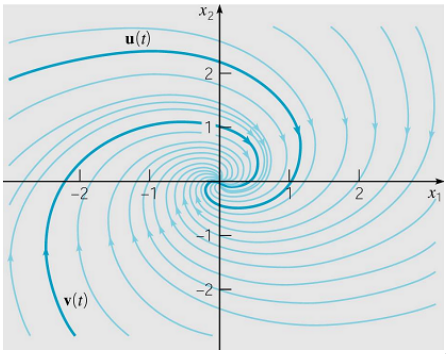
\includegraphics[width=0.45\textwidth]{figure/Lec13f2.PNG}
		\end{figure}
		\item The origin is a spiral point, and is asymptotically stable.
	\end{itemize}
	\section*{Example 1: Phase plane (7 of 8)}
	\begin{figure}[H]
		\centering
			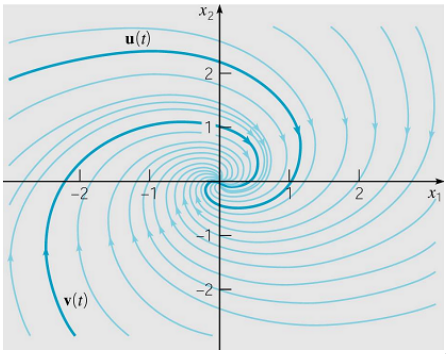
\includegraphics[width=0.65\textwidth]{figure/Lec13f2.PNG}
	\end{figure}
	\section*{Example 1: Time plots (8 of 8)}
	\begin{itemize}
		\item The general solution is $x = c_1u + c_2v$:
		$$
		x =
		\begin{pmatrix}
			x_1(t)\\
			x_2(t)
		\end{pmatrix}=
		\begin{pmatrix}
			c_1e^{-\nicefrac{t}{2}}\cos t + c_2 e^{-\nicefrac{t}{2}}\sin t\\
			-c_1e^{-\nicefrac{t}{2}}\sin t + c_2 e^{-\nicefrac{t}{2}}\cos t
		\end{pmatrix}
		$$
		\item As an alternative to phase plane plots, we can graph $x_1$ or $x_2$ as a function of $t$. A few plots of $x_1$ are given below, each one a decaying oscillation as $t \to \infty$.
		\begin{figure}[H]
			\centering
				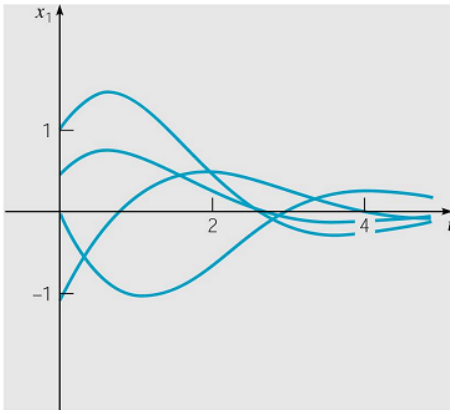
\includegraphics[width=0.40\textwidth]{figure/Lec13f3.PNG}
		\end{figure}
	\end{itemize}
	\section*{Spiral points, centers, eigenvalues, and trajectories}
	\begin{itemize}
		\item In previous example, general solution was
		$$
		x =
		\begin{pmatrix}
			x_1\\
			x_2
		\end{pmatrix} = c_1
		\begin{pmatrix}
			e^{-\nicefrac{t}{2}}\cos t\\
			-e^{-\nicefrac{t}{2}}\sin t
		\end{pmatrix} + c_2
		\begin{pmatrix}
			e^{-\nicefrac{t}{2}}\sin t\\
			e^{-\nicefrac{t}{2}}\cos t
		\end{pmatrix}
		$$
		\begin{figure}[H]
			\centering
				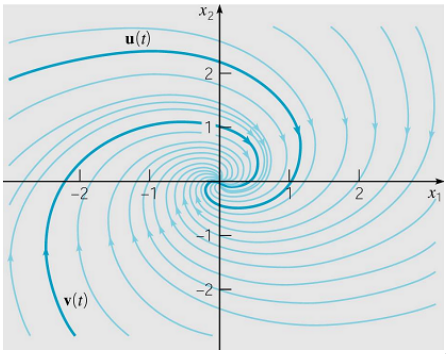
\includegraphics[width=0.45\textwidth]{figure/Lec13f2.PNG}
		\end{figure}
		\item The origin was a \textbf{spiral point}, and was asymptotically stable.
		\item If the real part of the complex eigenvalues is positive, then the trajectories spiral away, unbounded, from the origin, and hence the origin is an unstable spiral point.
		\item If the real part of the complex eigenvalues is zero, then the trajectories circle the origin, neither approaching nor departing. In this case the origin is called a \textbf{center} and is stable, but not asymptotically stable. These trajectories are periodic in time.
		\item The direction of trajectory motion depends on entries in \textbf{A}.
	\end{itemize}
	\section*{Second order solution behavior and eigenvalues: Three main cases}
	\begin{itemize}
		\item For second order ODE systems, the three main cases are:
		%
		\begin{itemize}
			\item[\labelitemi] Eigenvalues are real and have opposite signs; $x = 0$ is a saddle point.
			\item[\labelitemi] Eigenvalues are real, distinct and have same sign; $x = 0$ is a node.
			\item[\labelitemi] Eigenvalues are complex with nonzero real part; $x = 0$ a spiral point. 
		\end{itemize}
		%
		\item Other possibilities exist and occur as transitions between two of the cases listed above:
		%
		\begin{itemize}
			\item[\labelitemi] A zero eigenvalue occurs during transition between a saddle point and a node. Real and equal eigenvalues occur during transition between nodes and spiral points. Purely imaginary eigenvalues occur during a transition between asymptotically stable and unstable spiral points. 
			$$
			r = \frac{-b \pm \sqrt{b^2-4ac}}{2a}
			$$
			\begin{figure}[H]
				\centering
					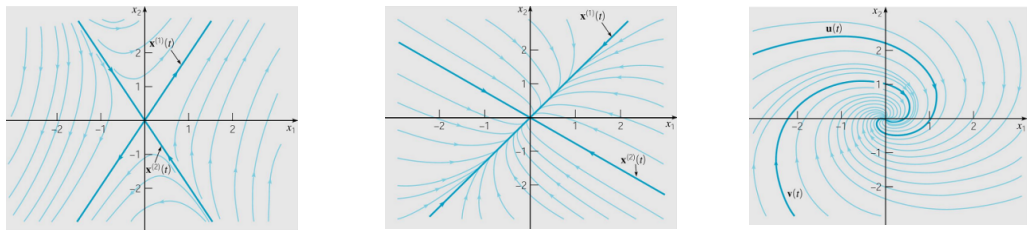
\includegraphics[width=0.80\textwidth]{figure/Lec13f4.PNG}
			\end{figure}
		\end{itemize}
		%
	\end{itemize}
\end{document}